\documentclass{article}

\usepackage{multirow}
\usepackage{arxiv}
\usepackage{amsmath}

\usepackage[utf8]{inputenc} % allow utf-8 input
\usepackage[T1]{fontenc}    % use 8-bit T1 fonts
\usepackage{hyperref}       % hyperlinks
\usepackage{url}            % simple URL typesetting
\usepackage{booktabs}       % professional-quality tables
\usepackage{amsfonts}       % blackboard math symbols
\usepackage{nicefrac}       % compact symbols for 1/2, etc.
\usepackage{microtype}      % microtypography
\usepackage{lipsum}		% Can be removed after putting your text content
\usepackage{graphicx}
\usepackage{doi}



\title{Carbon Renaissance Whitepaper 1.0}

\author{

 \href{https://orcid.org/0000-0000-0000-0000}{
\includegraphics[scale=0.06]{orcid.pdf}\hspace{1mm}Greg Darragh}\\
	Carbon Renaissance\\
	\texttt{greg@crc.eco} \\
\And	
 \href{https://orcid.org/0000-0000-0000-0000}{
\includegraphics[scale=0.06]{orcid.pdf}\hspace{1mm}Mick Viner-Smith}\\
	Carbon Renaissance\\
	\texttt{mick@crc.eco} \\	
\And
 \href{https://orcid.org/0000-0000-0000-0000}{
\includegraphics[scale=0.06]{orcid.pdf}\hspace{1mm}Ian C. Moore, PhD}\\
	Syscoin Researcher\\
	\texttt{imoore@syscoin.org} \\
	\And
	\href{https://orcid.org/0000-0000-0000-0000}{
\includegraphics[scale=0.06]{orcid.pdf}\hspace{1mm}Jagdeep Sidhu, MSc} \\
	Syscoin Core Developer\\
	Blockchain Foundry Inc.\\
	\texttt{jsidhu@blockchainfoundry.co} \\
}

\renewcommand{\shorttitle}{Carbon Renaissance}

\hypersetup{
pdftitle={Stochastic Properties of EIP-1559 Basefees},
pdfsubject={q-bio.NC, q-bio.QM},
pdfauthor={Ian C. Moore, Jagdeep Sidhu},
pdfkeywords={Carbon Sequestration, Carbon Offsetting, Social Credit, NFT},
}

\begin{document}
\maketitle

\begin{abstract}
We propose a Carbon offset design that creates natural economic incentives through business
processes tied to NFT tokens issued from enterprise to participating companies which connect
to Carbon offsetting processes. Upon audits of work, a fungible token (Green token) is issued to
companies involved based on a pre-negotiated ratio of tokens dispersed based on the quality of
the work and quality of the credit-worthiness of the companies involved. Green token supply
represents a collection and aggregation of all pollution prevention value that has happened thus
far.
\end{abstract}

\keywords{Carbon Sequestration \and Carbon Offsetting  \and Social Credit \and NFT}

\section{Executive Summary}
\subsection{Mission and Vision}

We propose a Carbon offset design that creates natural economic incentives through business
processes tied to NFT tokens issued from enterprise to participating companies which connect
to Carbon offsetting processes. Upon audits of work, a fungible token (Green token) is issued to
companies involved based on a pre-negotiated ratio of tokens dispersed based on the quality of
the work and quality of the credit-worthiness of the companies involved. Green token supply
represents a collection and aggregation of all pollution prevention value that has happened thus
far.

We extrapolate that this will not only allow for incentives to modify spending behaviour of
consumers but also produce an easy vehicle for companies to adhere to Carbon quotas by
purchasing and offsetting their carbon through a novel token model. Furthermore we extend to
assert that perhaps this essentially facilitates a Universal Basic Income model once we are able
to leverage blockchain for fair exchange of carbon tokens in auditable and censorship
resistance mediums.

\subsection{Problem Statement and Strategy}

There are a number of benefits that this Carbon offset model can provide. 

Token supply creation requires work, which include Carbon sequestration followed by an auditing process working with various stakeholders that are involved in the process. This minting of new token supply can be compared to Bitcoin's Proof-of-Work (PoW) process popularily described an \emph{mining}, which is a completely automated and trustless process. However, the CR token minting process is governed by a regulatory work-flow process working through various stakeholders. Many of the market dynamics that we know which drive price discovery via the Bitcoin miner network can be utilized to understand the market dynamics with this project. Such dynamics include: (a) geographical advantages characteristic to the local environment; (b) regulations particular to certain jurisdictions that allow for more cost effective sequestration; and (c) technological advancements.

The token supply can work in both a inflation/deflation environment depending on the system setup. Whereas other projects are either strictly deflationary or inflationary. For instance, we show via simulation that it is possible to have the supply reach a state of equilibrium where supply is constant.  This economic feature can make it attractive for large corporate organizations and governments to work with.

The CR process works in a cycle where the token can move to one of three different states over time (ie, statetokens). These states are: (a) Green; (b) Red; and (c) Black, and are usecase dependant. Green tokens (otherwise refereed as base tokens) are purchased on exchanges and represent the potential of what can be utilized for Carbon sequestration and are required to enter into the auditing process. Red tokens are non-tradable Non-Fungible Tokens (NFT) and represent unique IOU contracts between stakeholders who have intentions to sequester Carbon and those who offer the Carbon sequestration service; see Fig. \ref{fig:issue_redeem_green}. NFTs are unique digital assets that are stored on a blockchain and cannot be exchanged for one another, hence non-fungible. Finally, Black tokens represent sequestered Carbon. For instance, 100 Black tokens represent proof of 100 units of sequestered Carbon. These tokens are created when either Red or Green tokens are burned. Black tokens can be either held privately or can be publicly purchased on exchanges. Holding these tokens over time have the advantage of generating Green tokens which can generate additional revenue by being sold and recycled back into the system. We will be expounding further into the dynamics and utility behind these statetokens throughout this whitepaper.
 
\subsubsection{NFT Tokens}

NFT tokens represent legal contracts and partnership with NFT issuances. They have the ability to white and black list those issuances to control the conversions and have the authority to issue monetary redemptions of those NFT’s if they are breaking contract rules. Bundling these NFTs into these promissory contracts helps decouple concerns between pollution prevention companies and users of the credits. This idea allows stakeholders to seamlessly enable onboarding of partners without upfront costs. This disruptive technology allows for the seamless onboarding of partners without upfront costs and regulatory pressures that would otherwise slow down the workflow process using traditional means. Not requiring upfront investment and low barrier of entry for existing pollution prevention services will greatly increase the chance of network effects. Participants can target businesses by offering them the NFT and liquidity on the open market in exchange for their services. 

There is no responsiveness required on behave of pollution prevention service providers as they can do as little or as much work as they want. Hence, no queues needed and no required customer acquisitions. All provided services are compensated (ie, as long as it's audited and verified) and are motivated to be efficient by decoupling prevention of pollution from customer demand.

NFT tokens are minted upon the creation of each new contract which is a promissory note to sequester a pre-determined amount of Carbon. Once the obligation of NFT contract is fulfilled, Green tokens are issued in exchange for service provided which in turn increase Green token supply. However, overall Green supply increases when NFTs are minted, but not tradable Green tokens themselves. Hence, by definition total Green supply includes the aggregation of tradable Green tokens and non-tradable NFTs. Pre-negotiated rates (even in non-token values if needed) are possible between stakeholders and CR for NFT to Green coin exchange. This will give the ability to offload speculative concerns on the sequestration services part to CR. These speculative concerns can also be abated via raising capital to offer liquidity on the markets (ie, to buy Green tokens) when needed as well.

\subsection{Solutions: Social Credit}

Using a carbon token incentive system would redistribute wealth, incentivize low carbon
technology and avoid the environmental taxes which hit the world’s poor the hardest.

In some systems the proposed UBI solutions are targeted to close the segregation between
the rich and poor but come at the cost of political interference. However these systems
rarely work in practice because of the lobbying from the wealthy which have power to
unilaterally dismiss such systems that intend to close the gap through taxation on rich and
profitable corporations. Companies and people that move would ideally be met with similar
taxation systems in other jurisdictions however these other jurisdictions may or may not
comply depending on their own policies and mandates to grow local economies through
immigration of these wealthy people and companies.

Using our carbon offset token program way, governments can purchase carbon offsets
which are an efficient spend of budget against environmental impacts of its economy and
reduce taxes to those that inhibit green spending habits such as buying local and not going
over their carbon footprint quota per person. A positive reinforcement model will always be
unanimously acceptable to both the wealthy and the poor. Creating a positive feedback loop
to incentivize people to adapt their spending habits is a great way to find new efficiencies
and invent “greener” technologies due to the higher demand for such technologies and
services. The work here will be to assign carbon scores to goods and services and also
assign spending against carbon ratings of goods and services. People that have a negative
carbon footprint can be paid in Green tokens creating a powerful driver to reduce pollution
and assigning monetary benefits which can be part of a UBI system, one which is tied to
actual production and verified work.

\section{Proposed Design}

\subsection{Overview}

In the CR process, tokens move through a series of three states in an acyclic fashion. When the token is in a particular state, it can otherwise be defined as a Statetoken, and (as discussed in the previous section) can take on the characteristics of one of three forms (ie, Green, Red, and Black). Upon initial issuance, 100M Green tokens are issued by CR, and over time this supply is set to decrease, while the supply of Red and Black tokens rise from zero to some steady-state equilibrium over time. Fig \ref{fig:state_diagram} illustrates the state transition diagram where the nodes represent tokens and the arcs represent the direction and probability of a token transitioning to another over a unit of time.

Once the initial issuance of 100M Green tokens has occurred, then pollution prevention stakeholders are issued one NFT asset for each partner, with assigned value based on their risk profile. The assigned value of the NFTs is denominated in Green basecoins in the form of debt. This assigned value denominated Green tokens is based on the risk profile of the NFT holder (ie, akin to credit worthiness) which can be dynamically adjusted. These  pollution prevention stakeholders can assign tokens to various sequesters competing in various markets for those contract NFTs. Those NFTs, which have a unique value based on jurisdiction or cost, are sent to these sequesters and audited based on circumstances with those issuers and partner stakeholders.

The NFT stays in the possession of the sequesterer until the work has been performed and verified via the auditing process. Once complete, the NFT is burned and exchanged for both Black tokens as proof of sequestration and Green tokens which can be sold for revenue. Further to that, Black tokens can be held by sequesterer which when held over time slowly burn back into Green tokens. Each NFT may have its
own rules, regulations and even sequestering costs factoring in base asset to NFT cost ratios.

Burning Green directly tokens can also result Black tokens directly by entering into the auditing process to apply credit to the pollution prevention stakeholder. Once Green tokens are burned the holder will receive Black tokens. Holding these tokens is advantageous over extended periods of time, which will result in the minting or new Green tokens. For instance, if the state transition probability from Black to Green is 0.01, then 100 Black tokens will produce 1 Green token and 99 Black tokens when the state transitions across one unit of time.

Green token supply increases as sequestering happens and decreases as companies accumulate and burn Green tokens as proof that they have credits. If the rate of seqestration is exceeds the rate of credit consumed by companies then the Green token supply is inflationary and is deflationary if sequestering doesn’t adequately satisfy the burning of credits to black. For the deflationaray case, sequestering services will naturally start to fill the demand and organically find equilibrium.

\begin{figure}
\centering
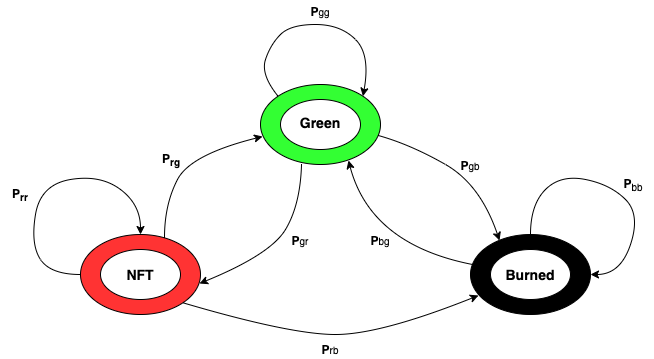
\includegraphics[width=4in]{state_diagram.png}
\caption{State transition diagram for Markov chain token model illustrating the probability of a token transitioning between states (ie, Green, NFT, and Burned) over a unit of time.} 
\label{fig:state_diagram}
\end{figure} 

\subsection{Benefits}

\begin{itemize}
\item Creates an analogous “miner” network, localized to jurisdiction or to company. Tap into
the work of others by infiltrating different geographic and types of sequestering for you,
even letting others race to acquire better sequestering techniques (like how bitcoin
miners raced to create asics). The more sequestoring they can do the more profits they
achieve.
\item Creates an inflation/deflation environment for Basecoin for a healthy market which is
realistic. One way deflationary markets suffer from utility concerns (first come first serve
won’t work here) and inflationary markets have little demand. One monetary instrument
for the entire system that simplifies economics and buy-in from government/enterprises
\item Allows separation of concerns between sequestoring companies and users of the
credits
\item Enabled onboarding of partners without upfront costs. Allows you as a company
facilitating the NFT to Basecoin conversions to issue new NFT’s strategically to
countries, businesses etc without requiring an upfront investment from those companies
(you can hold a deposit externally to avoid deadbeat companies that do not follow
through). Not requiring upfront investment and low barrier of entry for existing
sequestorers will greatly increase the chance of network effects. You can target any
business doing something like this and offer them the NFT and liquidity on the open
market in exchange for their services
\item Legal contracts and partnership with NFT issuances with ability to white/black list those
issuances to control the conversions and thus monetary redemptions of those NFT’s if
they are breaking contract rules
\item There is no responsiveness required on the sequestorers part. They can do as little or as
much work as they want, no queues needed and no required customer acquisitions. For
any work they do they should be paid (as long as it's audited and verified). The more
efficient their work becomes the more they can sequester and thus more they get paid.
The act of decoupling sequestoring from customer demand, makes the whole system
more efficient and greener
\item Works with any type of sequestoring model, each NFT can be uniquely identified in
terms of costs of base coin to NFT valuations based on the capture models storage vs
utility vs other
\item In order to mint new NFT’s, Basecoin supply increases but not the available supply (as
the NFT is not tradeable only the base coin is and thus the market cap of the base coin rises on issuances. The available supply increases when an NFT is burned in exchange
for Basecoin
\item Pre-negotiated rates (even in non-token values if needed) are possible between
partners/sequestorers and CR for NFT to Basecoin exchange. This will give ability to
offload speculative concerns on the sequestorer's part to CR, however CR can also raise
capital to offer liquidity on the markets as needed as well.
\end{itemize}

\subsection{Revenue Models}

\begin{itemize}
\item Percentage of profits on the NFT to Basecoin conversions for recurring revenue as a
platform as a service
\item CR sequestoring and earning Basecoin. Hold or sell
\item Value added services on top, softwares, wallets and other things some
companies/partners may pay extra for.
\end{itemize}

\subsection{Tokenized Company Shares}

It was requested that we create a fungible token for the purpose of share allocations in a
company represented as a token product on blockchain. Also these shares should not be
transferable unless explicitly allowed by CR. We can enable this functionality on Syscoin
through Notary services which will allow a case by case basis for transaction authorization
between P2P transfers. See spec:
https://github.com/syscoin/sips/blob/master/sip-0002.mediawiki

We should define the Maximum supply and precision as well as token symbol.
Token to sell to raise funds:
\begin{itemize}
\item Max supply: 100m
\item Precision: 8
\item Total raise: sell 10m upfront @ \$10
\item Token symbol: GCX
\end{itemize}

Token to issue as NFT for companies
\begin{itemize}
\item Max supply: MAX
\item Precision: 8
\item Token symbol: CX
\end{itemize}

Individual NFT:
\begin{itemize}
\item Precision: 8
\item Max supply: MAX
\end{itemize}


\subsection{Tokenomics}
\label{section:token_model}

Assume we are given the following stochastic (Markov) matrix:

\begin{equation*}
P = 
\begin{bmatrix}
p_{g,g} & p_{g,r}  & p_{g,b} \\
p_{r,g} & p_{r,r}  & p_{r,b} \\
p_{b,g} & p_{b,r} & p_{b,b} 
\end{bmatrix}
\end{equation*}

where each element is non-negative and each row sums to one. Each row of $P$ can be regarded as a probability mass function over $n$ possible outcomes. For instance, element $p_{g,b}$ represents the probability of a green token transitioning to a black token
between states. For our problem we setup the following transition matrix representing our business targets:

\begin{equation}
P_{\mu} = 
\begin{bmatrix}
0.95 & 0  & 0.05 \\
0.05 & 0.9  & 0.05 \\
0.01 & 0 & 0.99
\end{bmatrix}
\label{e:transition_matrix}
\end{equation}
where the frequency is monthly, and the states are represented as green, NFT, burned respectively. In Fig \ref{fig:gas}, we represent this Markov process as a directed graph with edges labelled by the transition probabilities in (\ref{e:transition_matrix}).

Let's assume $\{X_{t}\}$ is a Markov chain with stochastic matrix $P$, and the distribution of $X_{t}$ to be $\psi_{t}$. Hence, if we let the initial distribution of $\psi_{0} = [1,0,0]$, the probability distribution of $X_{t}$ can be determined via:

\begin{equation}
X_{t} \sim \psi_{0}P^{t}
\label{e:pow_vs_pos}
\end{equation}

Hence, the estimated token supply at time $t$ is given by:
\begin{equation}
\hat{S}_{t} = (S_{0} + \alpha N_{t})\psi_{0}P^{t}
\label{e:token_supply}
\end{equation}
where $S_{0}$ is the initial token supply (ie, 100M Green, 0 NFT and 0 Black tokens), $N_{t}$ represents the NFT IOU rate, and $\alpha \in [0,1)$ represents the global quality factor (eg, 0.9).

\subsubsection{Token Model Simulation}

To simulate transition probabilities in $\mathbf{P}_{t}$, we use the Beta distribution:
\begin{equation}
\mathbf{p}_{m,n,t} \sim Beta(\alpha_{m,n},\beta_{m,n})
\end{equation}
where $m$ is the current state, $n$ is the previous state and $\beta_{m,n} = 1-\alpha_{m,n}$. The parameters $\alpha_{m,n}$ and $\beta_{m,n}$ are selected such that $E\{\mathbf{P}_{t}\}$ = $P_{\mu}$. It is important to keep in mind that this is a stationary model, hence the expected values are invariant to time. We ensure that the rows of the simulations of $\mathbf{P}_{t}$ sum to one by applying the following normalization:
\begin{equation}
P_{m,n,t}'= \dfrac{P_{m,n,t} }{  \sum_{n} P_{m,n,t}  }.
\end{equation}
where $P_{m,n,t}$ represents the an element of $\mathbf{P}_{t}$ at time $t$. The simulated token supply  at time $t$ is defined as:
\begin{equation}
\hat{\mathbf{S}}_{t} =(S_{0} + \alpha N_{t})\psi_{0}\mathbf{P}_{t}^{t}
\label{e:token_supply_simulation}
\end{equation}


\begin{table}[h!]
\centering
\begin{tabular}{|c c|c|c|c| } 
\hline
 & \multicolumn{4}{ c |}{ Next State } \\
 &  & Green & NFT & Burned \\
\hline
\multirow{ 3}{*}{Current State} & Green & $P(X_{n+1} = g | X_{n} = g )$ & $P(X_{n+1} = r | X_{n} = g )$ & $P(X_{n+1} = b | X_{n} = g )$ \\
& NFT & $P(X_{n+1} = g | X_{n} = r )$ & $P(X_{n+1} = r | X_{n} = r )$ & $P(X_{n+1} = b | X_{n} = r )$ \\
& Burned & $P(X_{n+1} = g | X_{n} = b )$ & $P(X_{n+1} = r | X_{n} = b )$ & $P(X_{n+1} = b | X_{n} = b )$ \\
\hline
\end{tabular}
\caption{Transition state matrix for token model detailing probabilities of transitioning from current to next state over a unit of time. The token states are denoted by Green $\rightarrow$ g, NFT $\rightarrow$ r, and Burred $\rightarrow$ b.}
\label{table:pow_vs_pos}
\end{table}

\begin{figure}
\centering
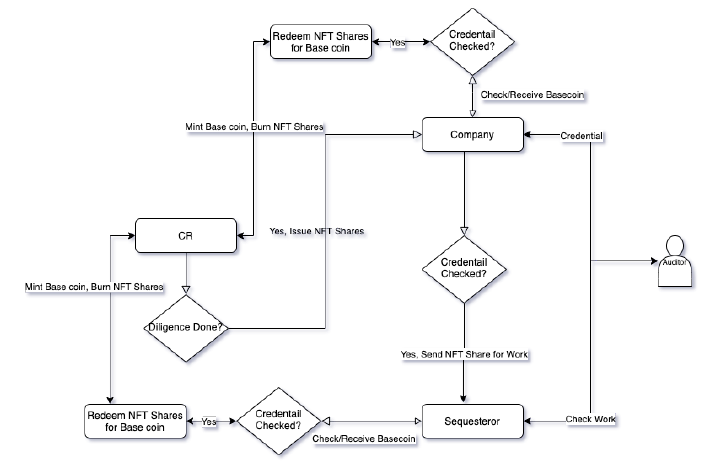
\includegraphics[width=4in]{issue_redeem_green.png}
\caption{xxx} 
\label{fig:issue_redeem_green}
\end{figure} 

\begin{figure}
\centering
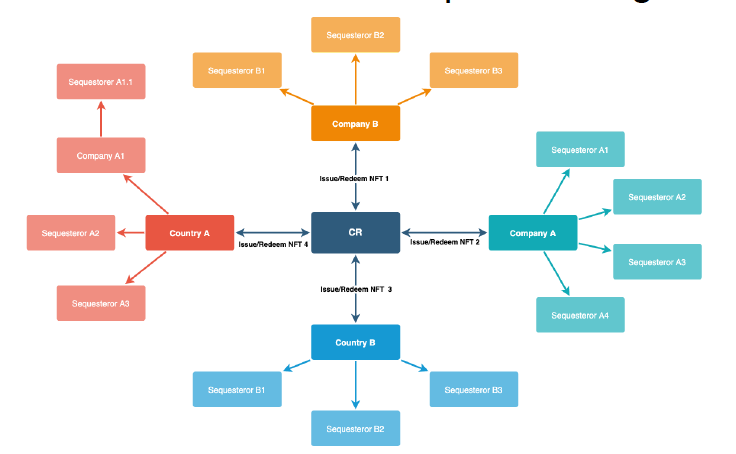
\includegraphics[width=4in]{red_green.png}
\caption{xxx} 
\label{fig:red_green}
\end{figure} 

\begin{figure}
\centering
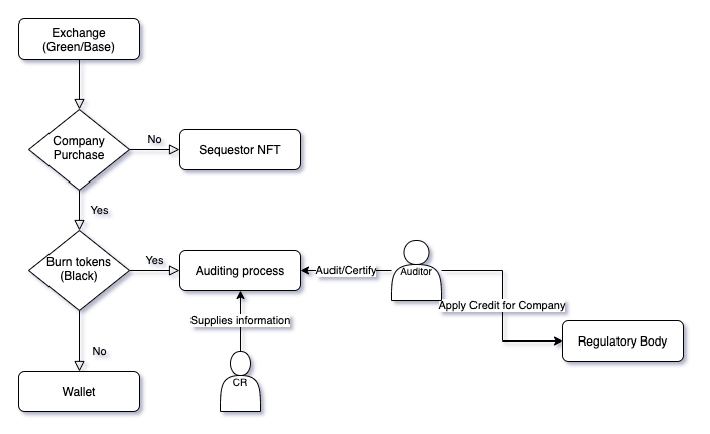
\includegraphics[width=4in]{green_black.png}
\caption{xxx} 
\label{fig:green_black}
\end{figure} 



\begin{figure}
\centering
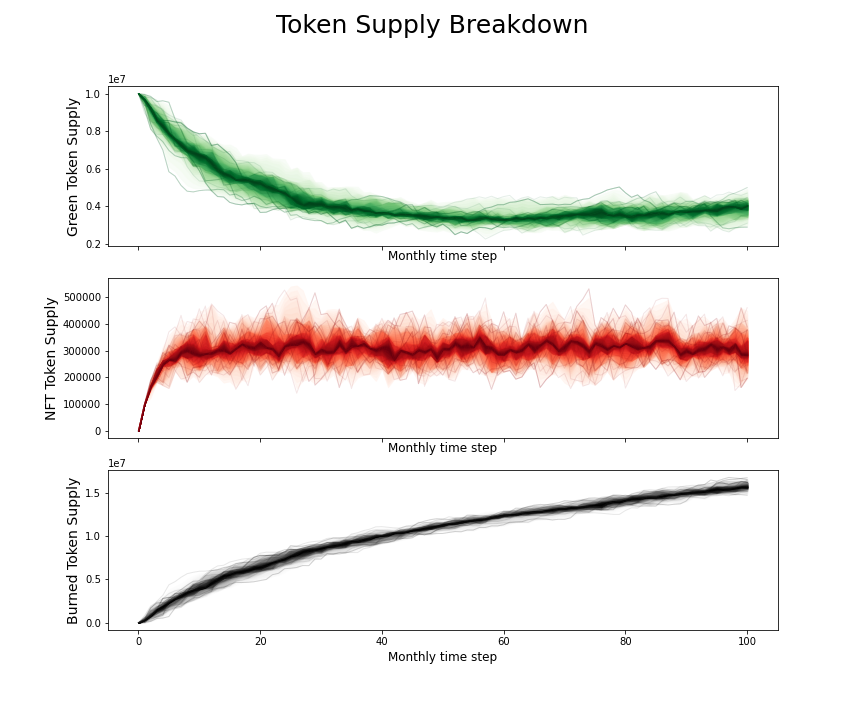
\includegraphics[width=4in]{token_supply_sims.png}
\caption{Markov Chain Token model simulations assuming stationary transition probabilities applying the Beta distribution at each time point at a monthly frequency. The expectations of the transition probability matrix was selected based on business targets. The simulation begins with 100M Green tokens, the bulk of which will transition to red and black tokens over time and eventually reach a state of equilibrium. When the system reaches steady-state the expected supply of each of the three tokens will remain constant.} 
\label{fig:token_supply_sims}
\end{figure} 

\begin{figure}
\centering
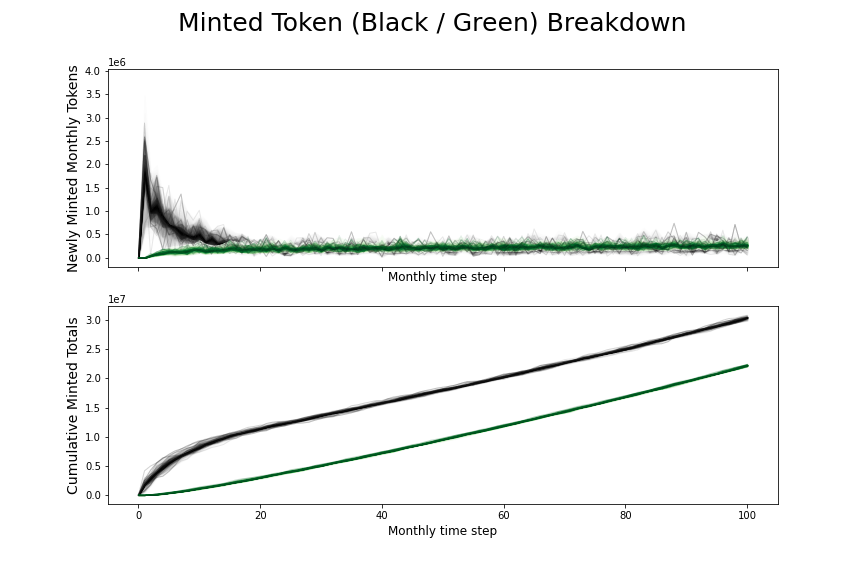
\includegraphics[width=4in]{burned_minted.png}
\caption{Newly minted green and burned tokens resulting from simulation model (\ref{e:token_supply_simulation}). Simulations of: (TOP) number of daily minted tokens; and (BOTTOM) cumulative number of daily minted tokens.} 
\label{fig:burned_minted}
\end{figure} 

\subsection{Revenue Model}

\begin{table}[h]
\centering
\begin{tabular}{ |c|c|c|c| } 
\hline
 Year & median & lwr 5\% & upr 5\% \\
\hline
1 & 4,730,000 & 3,080,000 & 6,230,000 \\
2 & 7,960,000 & 7,040,000 & 9,690,000 \\
3 & 11,000,000 & 9,800,000 & 12,260,000 \\
4 & 13,620,000 & 12,100,000 & 14,770,000  \\
5 & 16,060,000 & 15,120,000 & 19,710,000 \\
\hline
\end{tabular}
\caption{Simulated number of sequestered tons of Carbon assuming transition matrix (\ref{e:transition_matrix}) as business targets}
\label{table:pow_vs_pos}
\end{table}

\subsection{Token Architecture}

\section{Open Issues}

\subsection{Jurisdictional Requirements}

\begin{itemize}
\item What if companies need jurisdictional guarantees on sequestration to fulfill local
government driven quota’s.
\begin{itemize}
\item Companies can buy directly from a local sequestration provider, and buy their
NFT’s for a premium (to jump in front of a queue) and convert into Basecoin from
CR (pay requisite small fees for doing so) and then burn tokens through standard
means as discussed in the proposal. The deals would be directly with NFT
partners and sequestration companies and so are localized based on company
jurisdiction.
\item Companies alternatively can buy directly from CR to jump ahead of the audit trail
(aforementioned queue), which will put more demand on those jurisdictions to
produce more sequestration. This would be an option if enough sequestration is
available for example.
\item The premiums paid for these higher demands are not factored into the Basecoin
market unless the drivers of these markets push up price naturally as global
aggregate prices go up based on these drivers if they are big enough.
\end{itemize}
\item There would be a timestamped sequestration audit trail that goes on the blockchain and
accessible publicly (through hyperlink in the asset public data field). This would be a live
document that would update with signatures of auditors registered with Digital Identities
and timestamps of where/when they happened.
\item If companies require localized sequestration in exchange for burning Basecoin then
upon burn when the time stamped audit trail is updated to reflect “consumed”
sequestrations CR can simply pick and choose which sequestration’s to qualify for that
particular carbon credit application. Ie: if MSFT needs 100 tons American sequestration
only, and we have 100 tons of American sequestration in the audit trail, we can choose those sequestrations and label them as consumed. Future American sequestration
requests either need to pay the American sequestors or wait for more sequestrations to
register from American sequestors. Under normal circumstances the audit trail can be
consumed chronologically.
\item It would be ideal to have this a global thing under l'accord de Paris so that there are no
jurisdictional requirements because otherwise there is incentive to strike side-deals with
companies directly, if the sequestration is fungible it makes for more clear and
understandable usage of the system and a more stable supply/demand curve of Basecoin. It
is almost like the Euro currency, where multiple countries each with their own policies use a
single currency, it is not a total failure but better to have one policy that is applicable to avoid
chances of corruption. However it may not be up to us, and so we can employ this strategy
based on market research if required.
\item The timestamped log will bring about transparency between consumed sequestrations, the
actual registered audited sequestrations and allow one to audit that the supply of Basecoin’s
accurately represents the audited sequestration amounts since 1 Basecoin can represent a
certain amount of sequestration (per ton?). It will allow companies to know what is available
for consumption should there be requirements around jurisdictional consumption.
\end{itemize}

\subsection{Competition}

\subsection{Speculative vs Stable}

Proposed design is a mix of speculative for companies requiring credits (Basecoin) and Stable
(can set rates and offload speculative risks for companies dealing with sequestoring). While at
the same time allowing for parallelization of sequestoring for faster more responsive supply side
mechanics of Basecoin (carbon credits).

\begin{itemize}
\item 1 ton of carbon assigned amount of tokens (based on cost in \$)
\item Start 1 for 1 but over time as tokens become burned the ratio will change, 1 ton of
carbon will be less than 1 token
\item This model adds speculation and thus enterprises may buy and hoard tokens to reduce
their own costs over time and also for potential gains. The cost in \$ should remain
consistent however as the ratio drops on how many tokens required for 1 ton of carbon
emissions.
\item Is deflationary only and so has a supply/demand equilibrium problem
\end{itemize}

\subsubsection{Speculative}

\begin{itemize}
\item 1:1 ratio constant
\item Need to mint new tokens according to how many tons exist in the world, if amount being
sequestered globally is > than new pollution then tokens become deflationary, otherwise
it's inflationary
\item Can pollution be determined through census information that is dependable enough?
\item Over time the goal is for pollution to drop and thus supply to reduce. As the pollution
drops the cost per carbon to cleanup reduces?
\item So this removes speculation play on the token to make it friendly for enterprises to use
and buy only as required (not have to purchase in advance due to speculation
concerns).
\item This model assumes all global carbon credits are modelled in the supply/demand market
of the token. If global pollution is not modelled it is not 1:1 at scale.
\end{itemize}


\section{Summary}

Bitcoin miners themselves are under alot of pressure for polluting the environment to secure the
Bitcoin network. They can use such a system which is actually using Bitcoin’s PoW indirectly to
secure such a system but decreasing their carbon footprint. This may be something that miners
would be interested in consuming driving adoption and awareness.

Creating a standards body to work with stakefish/f2pool and other miners to find a way to
specify how carbon offsets can be applied to the industry effectively. How can “green”
tokenization work with existing market initiatives related to NFT and maybe even FT tokens?

Better understand AMM model pertaining to a more distributed system where sequestorers can
be direct to market. Understand the need for differing markets based on quality metrics.

Green purchase, burn to goto Red where there is a Queue in response to physical sequestoring
and Black once sequestering happens and Red is burned. In this model there is a direct relation
between purchase of green and sequestering. Is this a requirement? In the proposed design we
establish a more frictionless system but do not assume that there is a direct relation between
green Basecoin and sequestering (It is indirectly related through the network of sequestorers
that get paid Basecoin to do work). A queue system inherently decreases efficiency
exponentially to the number of parallel sequestorers as there needs to be coordination, and
delays as well as mapping of which sequestering is for who adds complexity overall.


\section{Research To-dos}

\begin{itemize}
\item \$10 per token to 1 ton of Carbon: needs research to determine costs
\item Carbon sequestration is subjective and no trust-less  as whole thing can be corrupted by few auditors
\begin{itemize}
\item need to think about concessions to be put in place to thwart these potential bad actors
\end{itemize}
\item Carbon sequestration work/costs is akin to electricity costs and different jurisdictions will have different sequestration costs
\end{itemize}


\label{section:summary}

\begin{thebibliography}{1}

\bibitem{Ali21} Ian Alison, \textit{Blockchain Coalition Launches Tradable Carbon Credit Token}, Accessed on: Jul 2021. [Online]. https://www.coindesk.com/blockchain-coalition-launches-tradable-carbon-credit-token

\bibitem{SolarCoin} \textit{SolarCoin is a cryptocurrency that incentivizes a solar-powered planet}, Accessed on: Jul 2021. [Online]. https://solarcoin.org/

\bibitem{AirCarbon} \textit{A digital exchange focused on eliminating market friction in a carbon constrained economy.}, Accessed on: Jul 2021. [Online]. https://www.aircarbon.co/

\bibitem{Carbonx} \textit{APersonal Carbon Trading Inc.}, Accessed on: Jul 2021. [Online]. hhttps://www.carbonx.ca/

\bibitem{Nori} \textit{The Nori Carbon Removal Marketplace}, Accessed on: Jul 2021. [Online]. https://nori.com/

\bibitem{Microsoft21} \textit{Microsoft Bought Carbon Credits Through Cosmos Blockchain}, Accessed on: Jul 2021. [Online]. https://thecoinshark.net/blockchain-news/microsoft-bought-carbon-credits-through-cosmos-blockchain

\bibitem{Pan19} Y. Pan, X. Zhanga, Y. Wanga, J. Yan, S. Zhou, G. Li, J. Bao, \textit{Application of Blockchain in Carbon Trading}, \emph{Energy Procedia}., vol. 1588, no. 7, Feb. 2019.

\end{thebibliography}



\end{document}
